\chapter[几何促进的3D分子图生成(GFMDiff)]{几何促进的3D分子图生成(GFMDiff)}
\label{chap:gfmdiff}

在本节中,本文将着重介绍3D分子生成的模型框架,具体包括本文提出的E(n)等变去噪内核,几何信息促进的损失函数,扩散及去噪过程和优化目标。本文提出的3D分子生成整体框架由图~\ref{fig:gfmdiff}所示。

\begin{figure}[h]
    \centering
    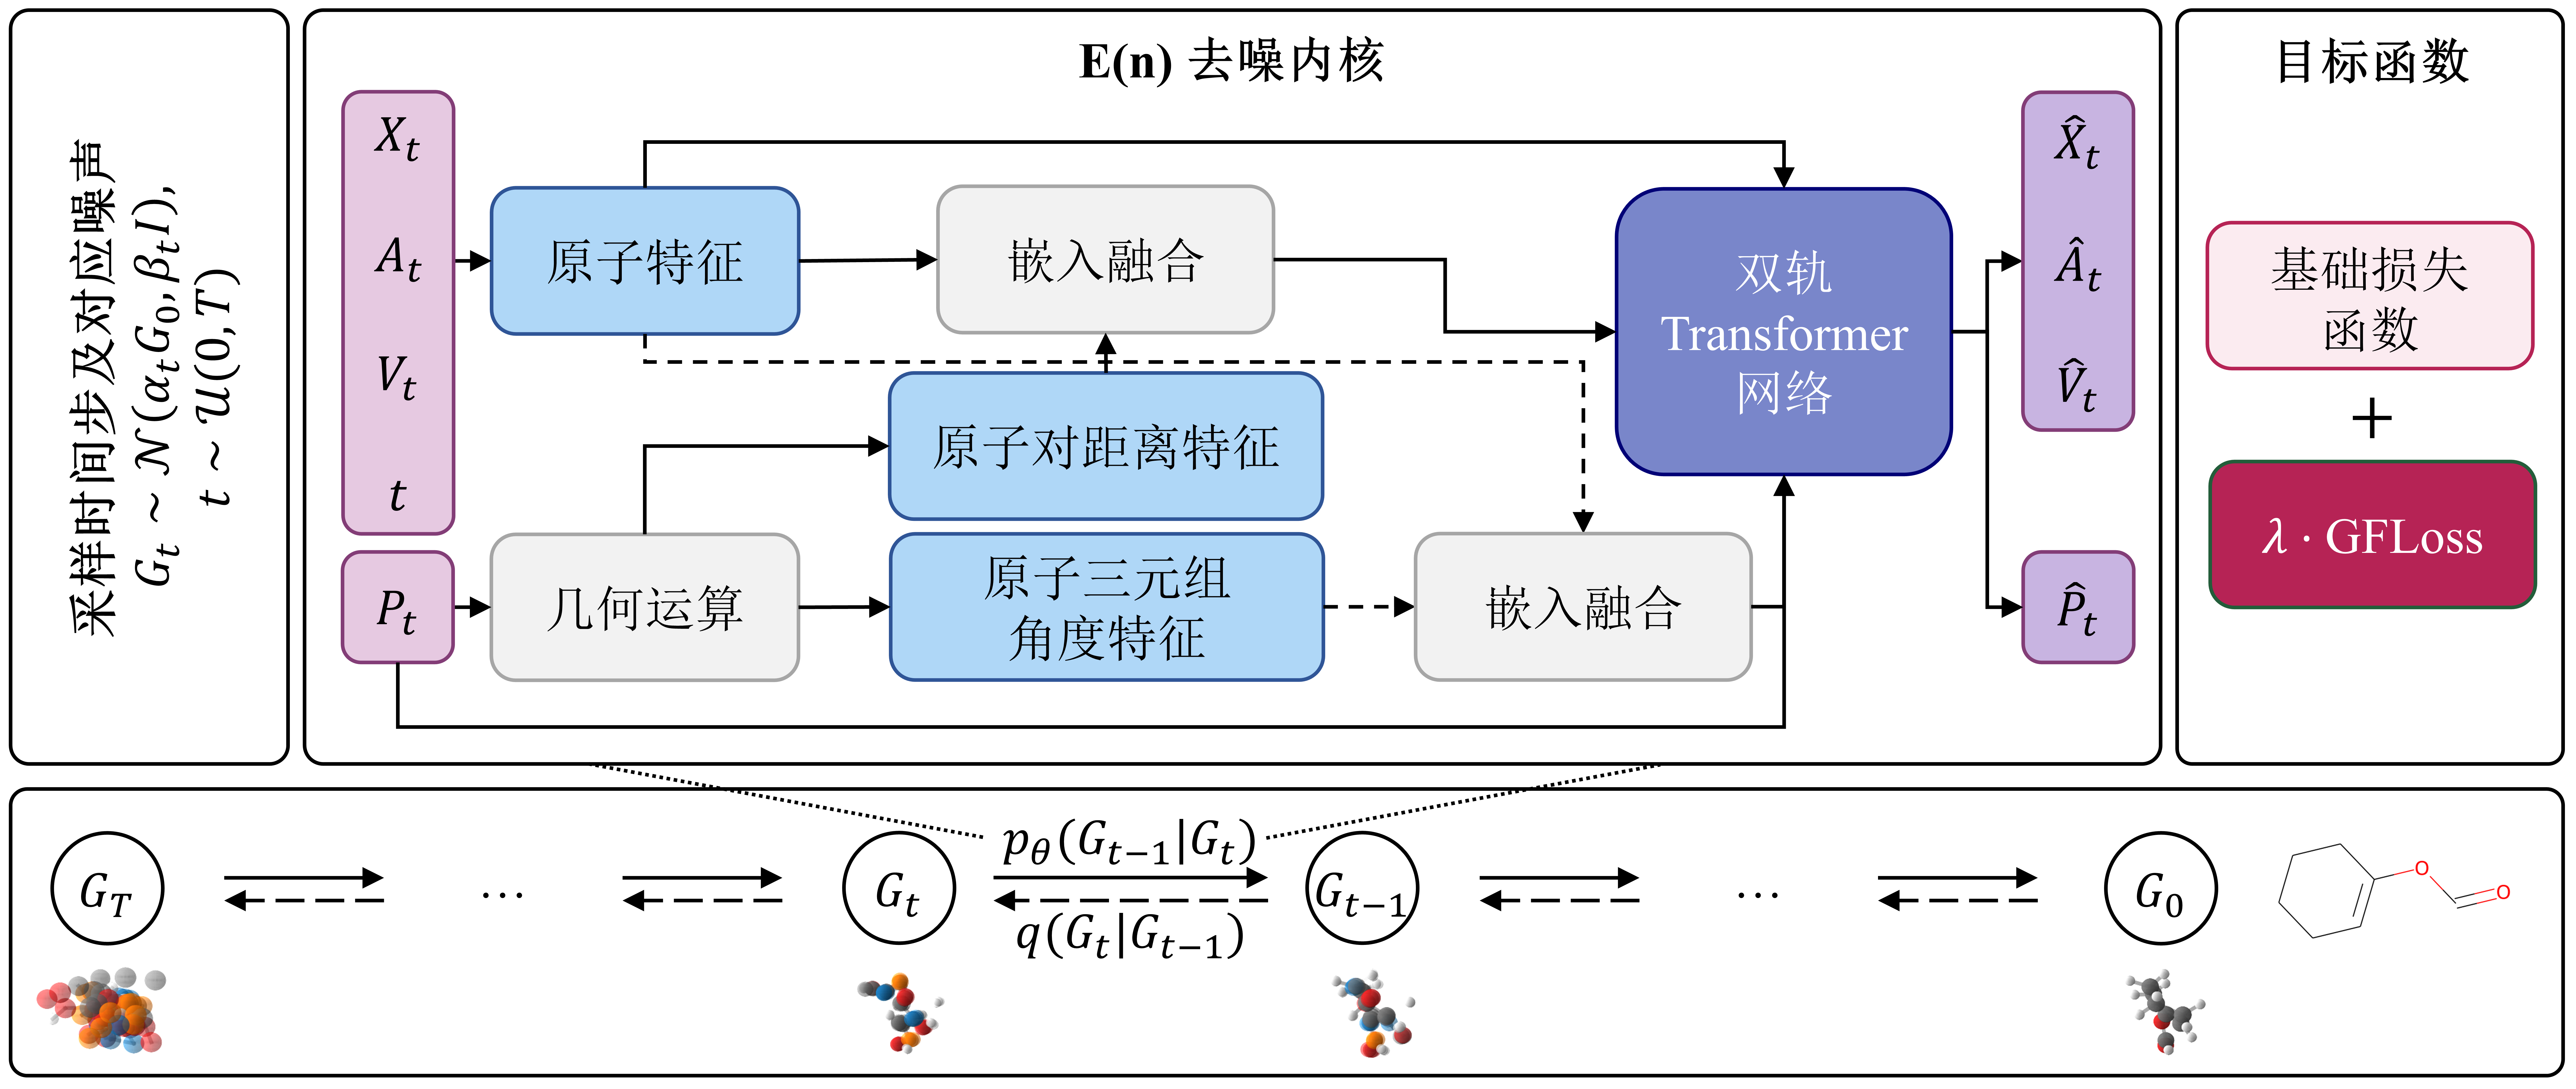
\includegraphics[width=\linewidth]{figures/overview_gfmdiff.png}
    \caption{GFMDiff模型框架示意图}
    \label{fig:gfmdiff}
  \end{figure} 

对于每个训练样本,模型的输入为随机选取的时间步$t$和采样自对应时刻噪声分布的样本。通过几何计算及编码,得到的原子特征,原子对距离特征,三元组角度特征将被用于E(n)等变的去噪内核DTN中的分子学习,并得到更新后的样本在$t-1$时刻的分布,即对应的原子特征和位置信息。

\section{双轨Transformer网络(DTN)}

在这个小节中,我们将详细介绍作为GFMDiff的E(n)等变去噪内核的双轨Transformer网络(Dual-track Transformer Network / DTN)。DTN被设计用于有效捕捉原子之间的关系和原子特征。由于三维分子几何具有旋转、平移、反射和排列等不变性质,使得去噪核满足这些性质是很重要的。所提出的DTN不仅是E(n)等变的,还能充分利用空间信息。

\begin{figure}[h]
  \centering
  
\includegraphics[width=\linewidth]{figures/structure_dtn.png}
  \caption{DTN去噪内核结构示意图}
  \label{fig:dtn}
\end{figure}

% 传统的图神经网络用于学习图结构数据的拓扑信息,仅仅是置换等变的。尽管已经有许多努力致力于赋予GNN上述性质,我们提供了另一种解决这个问题的视角。

在我们提出的方法中,我们将具有总原子数$N$的输入分子视为$G = (P, X, A, V)$,其中$P = (p_1, p_2, ..., p_N) \in \mathbb{R}^{N \times 3}$表示原子坐标,$X = (x_1, x_2, ..., x_N) \in \mathbb{R}^{N \times nf}$表示原子编号的独热编码,$A = (a_1, a_2, ..., a_N) \in \mathbb{R}^{N}$表示原子编号,$V = (v_1, v_2, ..., v_N) \in \mathbb{R}^{N}$表示原子的价数。为了确保等变性,DTN利用原子对距离信息和三元组角度信息捕捉几何信息。原子$i$和$j$之间的欧几里得距离反映了原子间相互作用的强度,可以通过以下公式获得:
\begin{equation}
    d_{ij} = ||p_i - p_j||_2.
\end{equation}
在分子中,除了氢原子,其他多数原子能够形成超过一个单键,故存在大量原子间的多体复杂关系。因此仅使用原子对距离是不足以充分提取空间几何信息。本文提出进一步使用以下公式计算三元角度:
\begin{equation}
    \varphi_{ijk} = \arccos (\frac{(p_i - p_j) \times (p_i - p_k)}{||p_i - p_j||_2 \times ||p_i - p_k||_2}). 
\end{equation}
经过上述几何计算,本文通过径向基神经网络(Radial Basis Function / RBF)编码得到可以被用作神经网络学习的原子对距离特征和三元组角度特征:
\begin{eqnarray}
    &e_{ij} = {\rm Linear}({\rm RBF}(d_{ij}), e_i, e_j),& \\
    &e_{ijk} = {\rm Linear}({\rm RBF}(\varphi_{ijk}), e_i, e_j, e_k),&
\end{eqnarray}
其中$e_i = {\rm Embedding}(x_i, a_i, v_i)$是原子$i$的节点嵌入,由原子序数和化合价决定。这些特征随后被输入到$L$层的DTN中。

DTN的每一层由以下组件组成:原子对轨道、对-三元轨道和连接模块。原子对轨道模拟了原子之间的相互作用力对目标原子的影响,而对-三元轨道模型则模拟了潜在键角对边的影响。连接模块作为两个轨道之间的桥梁,将原子特征注入到成对特征中,以促进更好的表示学习。

原子对轨道涉及预测其他原子和原子之间相互作用力对目标原子的影响。该轨道以原子嵌入$e_i$和对嵌入$e_{ij}$作为输入:
\begin{eqnarray}
    &e_i = {\rm LayerNorm}(e_i), \ e_{ij} = {\rm LayerNorm}(e_{ij}),& \\
    &\mathbf{Q}_i = {\rm Linear}(e_i), \ \mathbf{K}_i = {\rm Linear}(e_i) + {\rm Linear}(e_{ij}),& \\
    &a_i = {\rm Dropout}({\rm softmax} \frac{\mathbf{Q}_i \mathbf{K}_i^T}{\sqrt{d_h}}), & \\
    &\mathbf{V}_i = {\rm Linear}(e_{ij}) + {\rm Linear}(e_{i}) + {\rm Linear}(e_{j}),& \\
    &\hat{e}_i = {\rm Linear}(a_i \mathbf{V}_i^T),&
\end{eqnarray}
其中$d_h$是头的数量。原子嵌入首先通过添加原子对轨道的预测来更新,然后传递给前馈网络。在每一层中,原子吸收其他原子和相应的原子对的聚合表示。

类似地,对-三元轨道预测了复杂几何亚结构对原子间相互作用力的影响。
\begin{eqnarray}
    &e_{ij} = {\rm LayerNorm}(e_{ij}),&\\
    &e_{ijk} = {\rm LayerNorm}(e_{ijk}),&\\
    &\mathbf{Q}_{ij} = {\rm Linear}(e_{ij}),& \\ 
    &\mathbf{K}_{ij} = {\rm Linear}(e_{ij}) + {\rm Linear}(e_{ijk}),& \\
    &a_{ij}= {\rm Dropout}({\rm softmax} \frac{\mathbf{Q}_{ij} \mathbf{K}_{ij}^T}{\sqrt{d_h}}), & \\
    &\mathbf{V}_{ij} = {\rm Linear}(e_{ij}) + {\rm Linear}(e_{ijk}),& \\
    &\hat{e}_{ij} = {\rm Linear}(a_{ij} \mathbf{V}_{ij}^T).&
\end{eqnarray}
值得注意的是,三元嵌入$e_{ijk}$在Transformer结构中不会得到更新,因为这会显著增加计算资源的需求。它们只会在原子坐标更新时得到更新。

连接模块的作用是将原子嵌入融合到对嵌入中。对于对嵌入$e_{ij}$,它同时吸收来自连接模块的原子特征信息和来自对-三元轨道的局部空间信息。
\begin{equation}
    e_{ij} = {\rm LayerNorm}(e_{ij} + {\rm Linear}({\rm Linear}(e_i) \otimes {\rm Linear}(e_j)))
\end{equation}

在更新坐标的方法上,我们遵循EDM \cite{edm_hoogeboom_22}和MDM \cite{mdm_huang_23}的相关设计。由于原子坐标得到了更新,原子对和原子三元组的嵌入也将得到更新:

\begin{eqnarray}
  &e_{ij} = {\rm Linear}[{\rm Linear}({\rm RBF}(\hat{d}_{ij}), \hat{e}_{ij}), \hat{e}_i, \hat{e_j}],& \\
  &e_{ijk} = {\rm Linear}({\rm RBF}(\hat{\varphi}_{ijk}), e_{ijk}). &
\end{eqnarray}

\section{几何信息促进的损失函数(GFLoss)}
预测化学键的存在是分子图生成中的基本且不可或缺的任务。与以往的研究完全依赖于预设规则生成边不同,我们提出在训练过程中积极干预化学键的形成,通过设计一种精细的训练目标函数,命名为几何促进损失(Geometric-facilitated Loss / GFLoss)。这个损失函数的目的是引导模型生成既具有有效的拓扑结构,又具有稳定构象的分子。在分子生成中,我们认为原子的价是一种非常重要的辅助特征类型。因此,在上述提到的分子学习网络DTN中,原子的价被作为原子特征的一部分进行了整合。这使得模型能够学习和利用原子的价信息。

根据预定义的规则,具有适当距离的原子对被认为是由化学键连接的。对于单键、双键或三键,某些原子之间存在典型距离。如果一对原子之间的距离在某个范围内,这两个原子被认为是由对应类型的键连接的。假设预定义的距离和边界为 $\mathbf{D} \in \mathbb{R}^{nf \times nf \times 3}$ 和 $\mathbf{M} \in \mathbb{R}^{3}$,其中 3 表示键的类型数量。基于 DTN 的输出 $\hat{\mathcal{C}}_t = (\hat{P}_t, \hat{X}_t, \hat{A}_t, \hat{V}_t)$,我们首先使用 softmax 函数预测原子类型的概率:
\begin{equation}
    {\mathbf{p}}_t(\hat{X}_{{\rm atom}}) = {\rm softmax}(\hat{X}_t) \in \mathbb{R}^{N \times nf},
\end{equation}
其中 $\hat{X}_t$ 在此处表示维度为 $nf$ 的独热编码格式的预测原子类型。原子对的类型概率为
\begin{equation}
    {\mathbf{p}}_t(\hat{X}_{{\rm pair}}) = {\mathbf{p}}_t(\hat{X}_{{\rm atom}}) \cdot {\mathbf{p}}_t(\hat{X}_{{\rm atom}}) \in \mathbb{R}^{N \times N \times nf \times nf}.
\end{equation}

利用预测的原子坐标 $\hat{P}_t$,可以得到原子对之间的距离矩阵 $\mathbf{d}_t \in \mathbb{R}^{N \times N}$,并将其扩展为方便操作的 $\mathbb{R}^{N \times N \times nf \times nf \times 3}$。然后,原子对之间的距离与典型的键距离之间的边界 $\mathbf{m}_t$ 计算如下:
\begin{equation}
    \mathbf{m}_t = \mathbf{d}_t - (\mathbf{D} + \mathbf{M}) \in \mathbb{R}^{N \times N \times nf \times nf \times 3}.
\end{equation}
以原子 $i$ 和 $j$ 为例,假设它们被认为是碳原子的概率大于零,如果边界 $\mathbf{m}_t(i,j,{\rm C},{\rm C},:)$ 中的任何元素小于零,则表示原子 $i$ 和 $j$ 之间存在一条键。键的具体类型由边界 $\mathbf{m}_t(i,j,{\rm C},{\rm C},:)$ 中最小值的索引确定。如果 $\arg\min (\mathbf{m}_t(i,j,{\rm C},{\rm C},:))$ 为 1,则它们由一条单键连接。如果 $\arg\min (\mathbf{m}_t(i,j,{\rm C},{\rm C},:))$ 为 3,则它们由一条三键连接。表示键的布尔矩阵记为 ${\rm ISBOND}_t \in \mathbb{R}^{N \times N \times nf \times nf}$。

一旦我们获得了原子对的类型概率和键的存在情况,就可以估计原子的可能价:
\begin{equation}
     \hat{V}_{{\rm pred}}(t) = {\rm sum}({\mathbf{p}}_t(\hat{X}_{{\rm pair}}) \odot {\rm ISBOND}_t) \in \mathbb{R}^{N}.
\end{equation}
由于输入数据受到不同水平噪声的影响,GFLoss 被定义为预测价 $V_{{\rm pred}}$ 与真实价 $V$ 之间的均方误差:
\begin{equation}
    \mathcal{L}_{GF}(t) = ||\alpha_t(\hat{V}_{{\rm pred}}(t) - V_t)||^2,
\end{equation}
其中 $\alpha_t$ 是扩散过程中噪声数据中真实数据的水平。

\section{扩散及去噪过程}

在提出的GFMDiff的前向过程中,位置、原子序数和原子价逐渐被噪声先验分布所污染。通过具有预定义方差调度$\beta_t \in (0, 1), t=0, 1, ..., T$的马尔可夫链将真实构象$G_0 = (P_0, X_0, A_0, V_0)$进行转换。后验分布定义为:
\begin{eqnarray}
    &q(G_{1:T}|G_0) = \prod^T_{t=1} q(G_t|G_{t-1}),& \\
    &q(G_t|G_{t-1}) = \mathcal{N}_p(p_t;\sqrt{\alpha_t} p_{t-1}, \beta_t I) \cdot \\
    & \quad \quad \quad \quad \quad \mathcal{N}_h(h_t;\sqrt{\alpha_t} h_{t-1}, \beta_t I),&
\end{eqnarray}
其中$h_t = {\rm concat}(x_t, a_t, v_t)$表示原子特征,为了方便起见。为了满足等变性的要求,在将原子坐标引入扩散之前,它们必须先转换为线性子空间,其中质心为零\cite{enf_satorras_21,edm_hoogeboom_22,geodiff_xu_22}。因此,噪声分布和上述后验分布都受限于相同的线性子空间。虽然原子特征对于变换是不变的,但它们在整个前向和后向过程中与位置按相同的比例进行转换。

在去噪过程中,我们使用上述的去噪核函数来逼近每个时间步的分子构象,
\begin{eqnarray}
    &p_\theta(G_{t-1}|G_t) = \mathcal{N}(G_{t-1}; \mu_\theta(G_t,t),\sigma_t^2 I),& \\
    &\hat{G}_t = G_t / \alpha_t - \hat{\epsilon}_t * \sigma_t / \alpha_t ,&
\end{eqnarray}
其中$\hat{\epsilon}_t$是参数化神经网络的输出。

\section{目标函数}

对于DDPMs,典型的目标函数是数据对数似然的变分下界。在前人的方法基础上,我们将目标函数与GFLoss相结合:
\begin{equation}
    \mathcal{L}_t = E_{\epsilon_t \sim \mathcal{N}(0, I)}[\frac{1}{2}\omega(t)||\epsilon_t - \hat{\epsilon}_t||^2 + \lambda ||\alpha_t(\hat{V}_{pred}(t) - V_t)||^2],
\end{equation}
其中$\omega(t) = (1-{\rm SNR}(t)/{\rm SNR}(t-1))$。
